%% LyX 2.0.1 created this file.  For more info, see http://www.lyx.org/.
%% Do not edit unless you really know what you are doing.
\documentclass[english,t]{beamer}
\usepackage{lmodern}
\usepackage[T1]{fontenc}
\usepackage[latin9]{inputenc}
\usepackage{listings}
\lstset{basicstyle={\sffamily\small},
breakatwhitespace=true,
breaklines=true,
captionpos=b,
commentstyle={\color{red}\emph},
escapeinside={\%*}{*)},
frameshape={RYR}{y}{y}{RYR},
identifierstyle={\color{black}\bfseries},
keywordstyle={\color{blue}\bfseries},
numbers=none,
numbersep=5pt,
numberstyle={\color{black}\tiny},
showspaces=false,
showstringspaces=false,
showtabs=false,
stepnumber=1,
stringstyle={\ttfamily\color{red}\bfseries\emph},
tabsize=2}
\setlength{\parskip}{\medskipamount}
\setlength{\parindent}{0pt}
\synctex=-1
\usepackage{color}
\usepackage{babel}
\usepackage{float}
\usepackage{amsmath}
\usepackage{amssymb}
\usepackage{graphicx}
\ifx\hypersetup\undefined
  \AtBeginDocument{%
    \hypersetup{unicode=true,
 bookmarks=true,bookmarksnumbered=false,bookmarksopen=false,
 breaklinks=false,pdfborder={0 0 0},backref=false,colorlinks=false,pdftitle={RACE: Platforms and State of Simulation},
 pdfauthor={Sebastian Rockel, Denis Klimentjew},
 pdfsubject={RACE Kick-off Meeting, Dezember 2011},
 pdfkeywords={Robot, PR2, ROS, Restaurant}}
  }
\else
  \hypersetup{unicode=true,
 bookmarks=true,bookmarksnumbered=false,bookmarksopen=false,
 breaklinks=false,pdfborder={0 0 0},backref=false,colorlinks=false,pdftitle={RACE: Platforms and State of Simulation},
 pdfauthor={Sebastian Rockel, Denis Klimentjew},
 pdfsubject={RACE Kick-off Meeting, Dezember 2011},
 pdfkeywords={Robot, PR2, ROS, Restaurant}}
\fi

\makeatletter
%%%%%%%%%%%%%%%%%%%%%%%%%%%%%% Textclass specific LaTeX commands.
 % this default might be overridden by plain title style
 \newcommand\makebeamertitle{\frame{\maketitle}}%
 \AtBeginDocument{
   \let\origtableofcontents=\tableofcontents
   \def\tableofcontents{\@ifnextchar[{\origtableofcontents}{\gobbletableofcontents}}
   \def\gobbletableofcontents#1{\origtableofcontents}
 }
 \long\def\lyxframe#1{\@lyxframe#1\@lyxframestop}%
 \def\@lyxframe{\@ifnextchar<{\@@lyxframe}{\@@lyxframe<*>}}%
 \def\@@lyxframe<#1>{\@ifnextchar[{\@@@lyxframe<#1>}{\@@@lyxframe<#1>[]}}
 \def\@@@lyxframe<#1>[{\@ifnextchar<{\@@@@@lyxframe<#1>[}{\@@@@lyxframe<#1>[<*>][}}
 \def\@@@@@lyxframe<#1>[#2]{\@ifnextchar[{\@@@@lyxframe<#1>[#2]}{\@@@@lyxframe<#1>[#2][]}}
 \long\def\@@@@lyxframe<#1>[#2][#3]#4\@lyxframestop#5\lyxframeend{%
   \frame<#1>[#2][#3]{\frametitle{#4}#5}}
 \def\lyxframeend{} % In case there is a superfluous frame end

%%%%%%%%%%%%%%%%%%%%%%%%%%%%%% User specified LaTeX commands.
\usepackage[ uniWZ, tams, blockBG, engl, conference]{tamsBeamer}
%-- options	------------------------------------------------------
%	tams	|	- TAMS		publication
%	engl		- english strings	[german]
%	uniWZ	|	- uni		watermark
%	tamsWZ	|	- tams+uni	watermark
%	cinacsWZ	- cinacs+uni	watermark
%	secToc	|	- toc repetition at each section
%	secTocA		- -"-, all sections: show
%			  replacement for toc in short docs
%	subsecToc	- toc repetition at each subsection
%	secNum  	- (sub)-section numbering
%	fullstep	- always step through items
%	noFoot		- footline	off
%	noPage		- page numbers	off
%	noAuth		- author	off
%	conference	- footline with \foottitle{...}
%	blockBG	|	- block, example etc. background
%	blockRound	- -"-, rounded+shadow

\makeatother

\begin{document}







\title[Platforms and Simulation]{Platform(s) and State of Simulation}


\author[S. Rockel, D. Klimentjew, J. Zhang]{S. Rockel, D. Klimentjew, J. Zhang\textbf{}\\
{\small \{rockel, klimentjew, zhang\}@informatik.uni-hamburg.de\vspace{-1em}
}}


\date{
\includegraphics[width=0.13\paperwidth]{images/RACE_Logo_framed}\\
\today}

\makebeamertitle
%\pgfdeclareimage[height=0.5cm]{institution-logo}{institution-logo-filename}
%\logo{\pgfuseimage{institution-logo}}

\AtBeginSubsection[]{
  \frame<beamer>{ 
    \frametitle{Outline}   
    \tableofcontents[currentsection,currentsubsection] 
  }
}

%\beamerdefaultoverlayspecification{<+->}





\lyxframeend{}\lyxframe{Outline}

\tableofcontents{}


\lyxframeend{}



\section{Platforms}
\subsection{PR2 Introduction}
\begin{frame}
  \frametitle{Introduction}
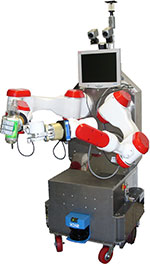
\includegraphics[width=2cm]{img/taser.jpg}
\hspace{5ex}
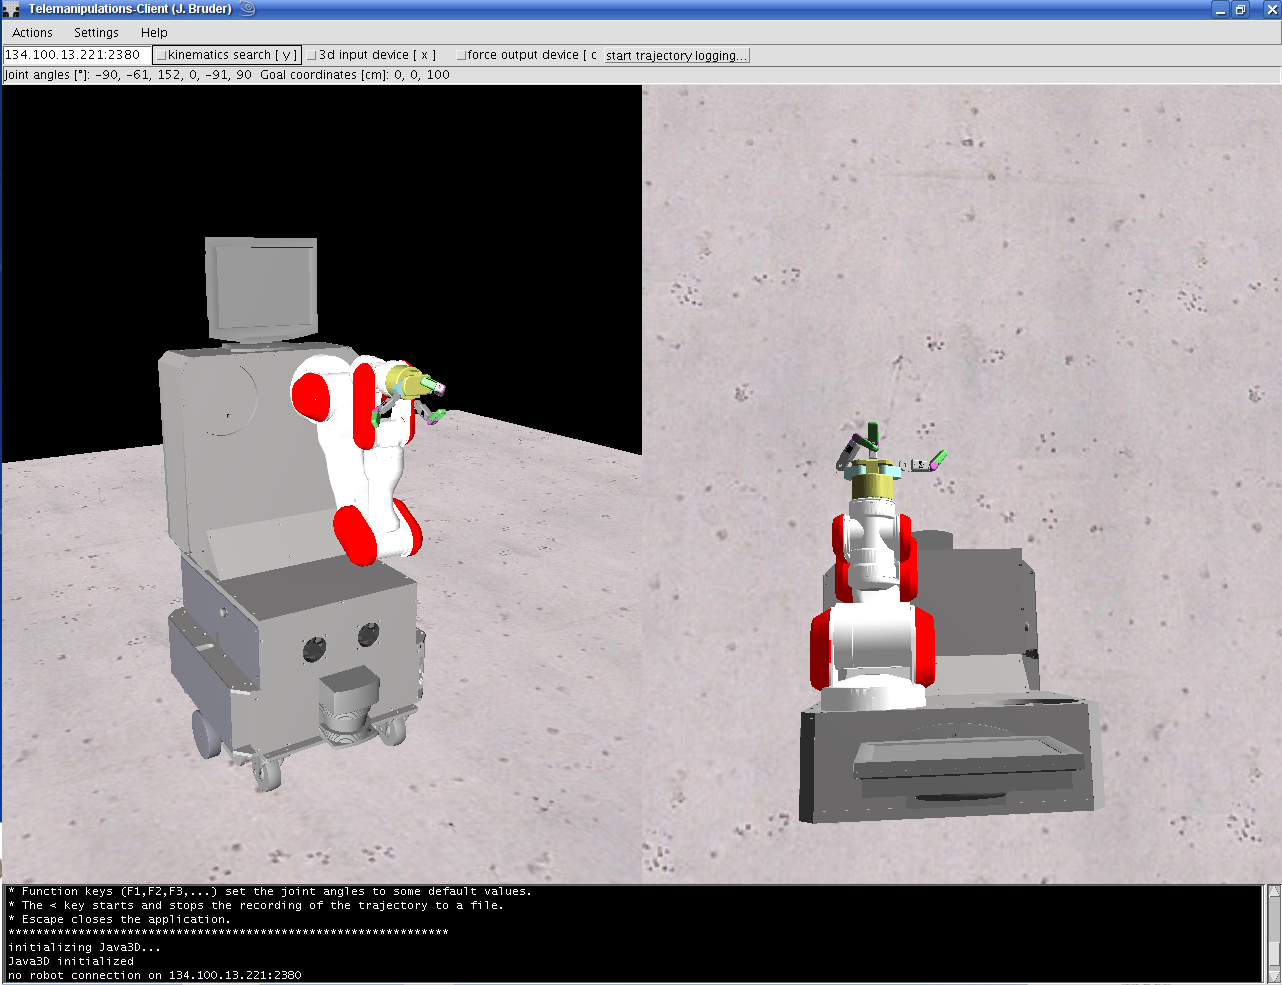
\includegraphics[width=5cm]{img/TASER_simulator1.png} \\[0cm]
\vspace{-6ex}
\hspace{33ex}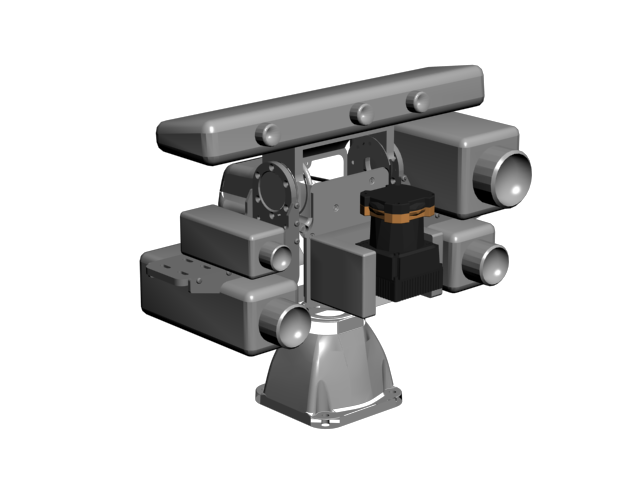
\includegraphics[width=5cm]{img/ActivePerceptionStereoHead_Top_Front.png}
\end{frame}


\subsection{PR2 Overview}
\begin{frame}
  \frametitle{PR2}
\hspace{-3ex}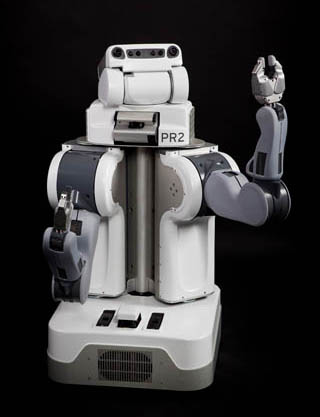
\includegraphics[width=3cm]{img/PR2_front.jpeg} 
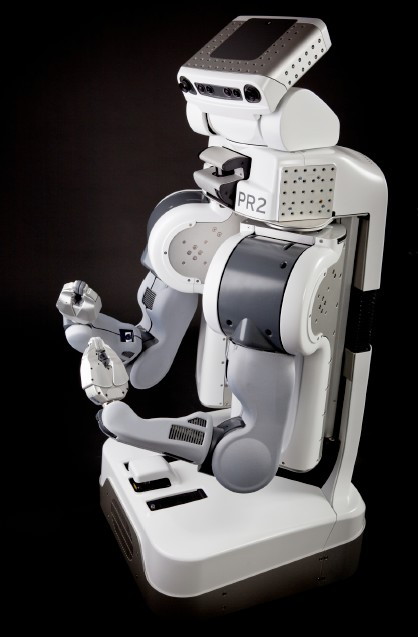
\includegraphics[width=2.57cm]{img/PR2_side.jpeg} 
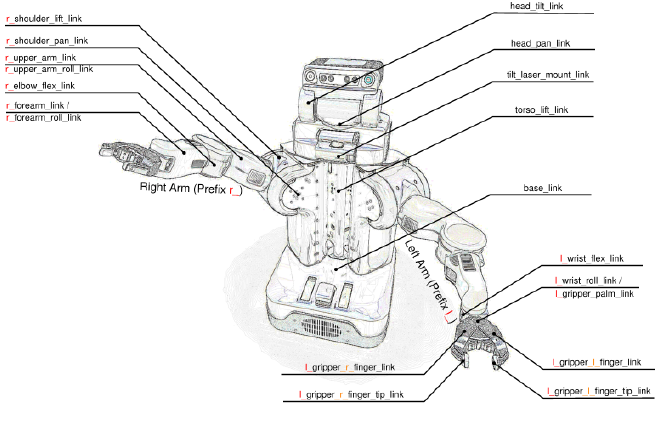
\includegraphics[width=6cm]{img/pr2_link_name.png}
\end{frame}

\begin{frame}
  \frametitle{PR2 - Users}
\centering\includegraphics[width=12cm]{img/pr2_users.pdf} 
\end{frame}

\begin{frame}
  \frametitle{PR2 - Hardware Specification}
\begin{itemize}
    \item $2\times$ computers with 24 Gb RAM and quad-core Nehalem processors
    \item 1.3 kWh Lion Battery Pack
    \item 2 hrs Approximate Runtime
    \item Coordinate system (for all links) positive z-axis up, positive x-axis forward, and positive y-axis robot-left when PR2 in the home pose
    
\end{itemize}
\end{frame}


\begin{frame}
  \frametitle{The PR2 motion control layout}
\hspace{15ex}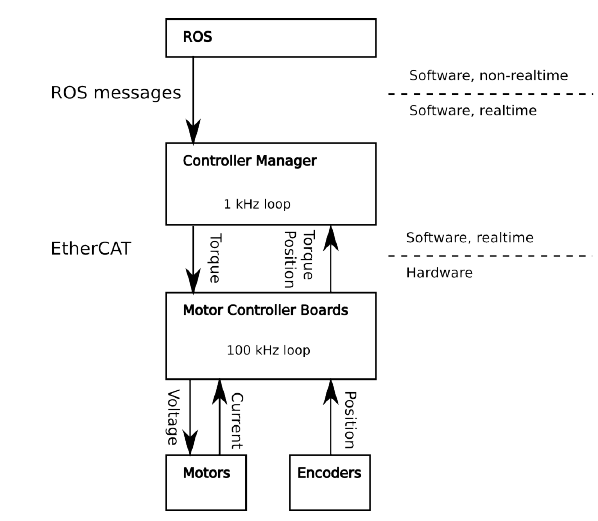
\includegraphics[width=7cm]{img/motion_control.png} 
\end{frame}

\begin{frame}
  \frametitle{Network explanation}
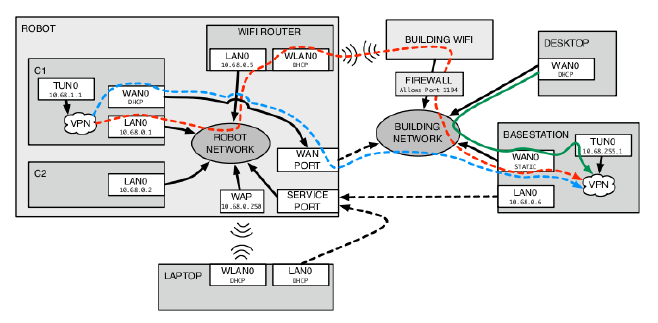
\includegraphics[width=12cm]{img/network.png} 
\end{frame}


\begin{frame}
  \frametitle{PR2 - Hardware Specification}
\small{
\begin{itemize}
    \item Arm DOFs: arm 4 (A), wrist 3 (B), gripper 1 (C)
    \item Link Lengths: upper arm 400\,mm, forearm 321\,mm,\\ wrist to gripper surface 120 - 200\,mm
    \item Range of motion: shoulder pan/tilt $170^0/115^0$,\\ upper arm roll $270^0$, elbow flex $140^0$, forearm \\roll continuous, wrist pitch/roll $130^0$/continuous, \\gripper 90\,mm max
    \item Force output: 4 DOF passive counterbalance, \\arm payload 1.8\,Kg, wrist torque 4\,Nm, \\grip force 80\,N
    
\end{itemize}
}
\vspace{-13ex}\hspace{47ex}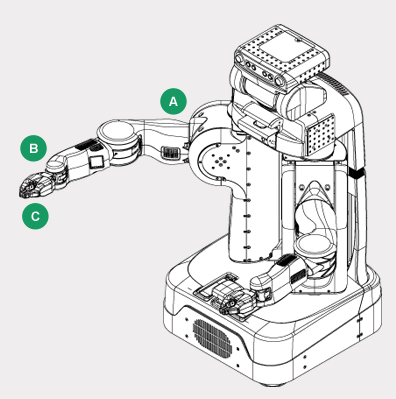
\includegraphics[width=3.4cm]{img/pr2_arm.png} 
\end{frame}

\begin{frame}
  \frametitle{PR2 - Intrinsic sensors}
\begin{itemize}
    \item Microstrain 3DM-GX2 IMU (above the shoulders)
    \item Three-Axis Accelerometer (gripper)
    \item Calibration LED (gripper) 
\end{itemize}
\end{frame}

\begin{frame}
  \frametitle{PR2 - Extrinsic sensors - Head}
\begin{itemize}
    \item Microsoft Kinect (color/depth image/point cloud $[640\times480 @ 30\,fps]$)
    \item Global shutter color gigabit ethernet camera (Prosilica GC2450C, 5\,MP, $[2448\times2050 @ 15\,fps]$)
    \item Wide stereo camera system (Aptina MT9V032C12STC, 100\,Mb color ethernet, $[752\times480@15\,fps]$)
    \item Narrow stereo system (Aptina MT9V032C12STM, 100\,Mb monochrome ethernet, $[752\times480@15\,fps]$)    
    \item LED textured light projector (triggered with narrow-angle stereo camera)
\end{itemize}
\end{frame}

\begin{frame}
  \frametitle{PR2 - Extrinsic sensors - II}
\begin{itemize}
    \item Tilting laserscanner (Hokuyo UTM-30LX, $135^0 (+90^0 to -45^0)$,above the shoulders)
    \item Laserscanner (Hokuyo UTM-30LX, base)
    \item Global shutter gigabit ethernet camera ($2\times$, forearm)
    \item Fingertip pressure sensor arrays (gripper)
    \item Speaker
\end{itemize}
\hspace{-4ex}
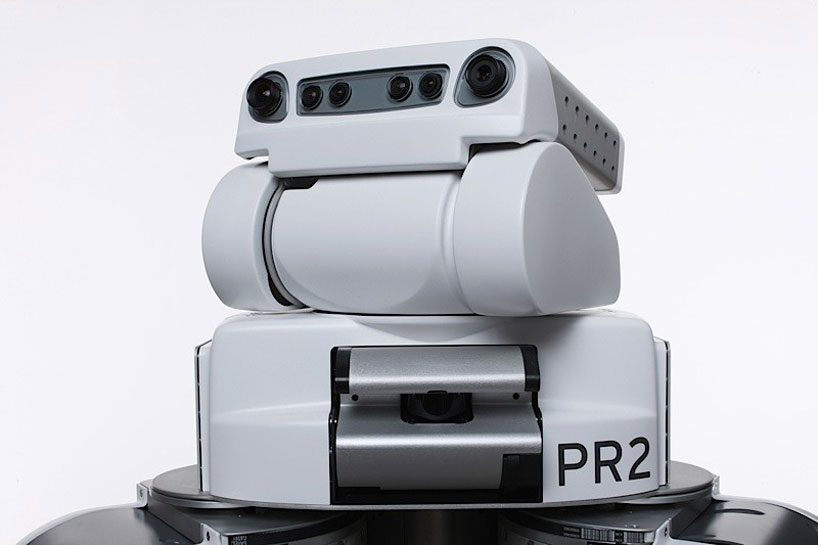
\includegraphics[width=4cm]{img/head_tiltLRF.jpg} 
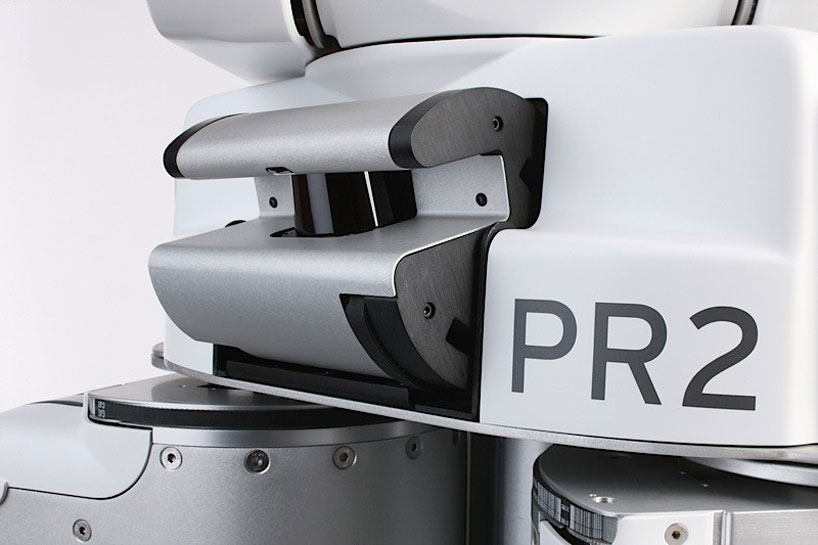
\includegraphics[width=4cm]{img/tilted_lrf.jpg}
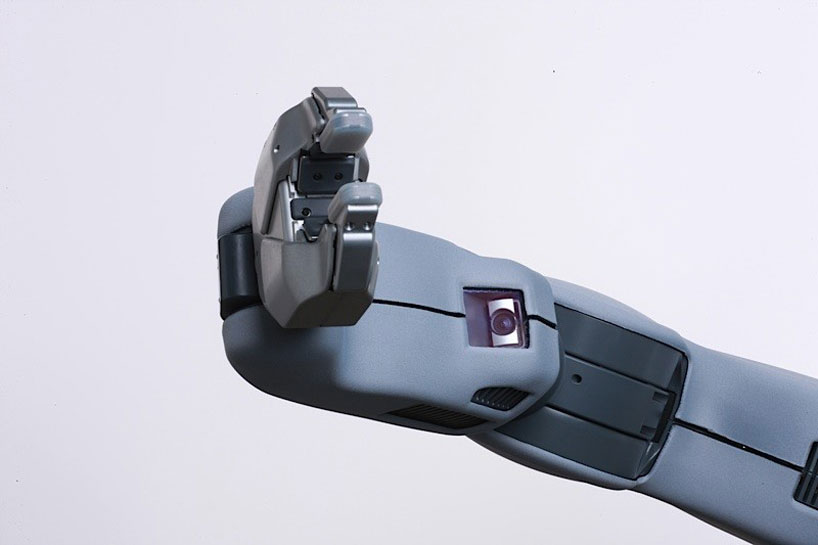
\includegraphics[width=4cm]{img/pr2_hand_camera.jpg}  
\end{frame}





\lyxframeend{}\section{ROS}


\lyxframeend{}\subsection{ROS Introduction}


\lyxframeend{}\lyxframe{ROS Introduction}

ROS
\begin{itemize}
\item Meta operating system for robotics
\item Obtain, build, write and run code across multiple computers and robots
\item Open source
\item BSD licensed (very liberal%
\footnote{\href{http://en.wikipedia.org/wiki/BSD_licenses}{http://en.wikipedia.org/wiki/BSD\_{}licenses}%
})
\item Willow Garage
\item Community
\end{itemize}

\lyxframeend{}


\lyxframeend{}\lyxframe{Introduction (cont.)}


\framesubtitle{Robots Using ROS > 50}

\noindent \begin{center}
\begin{figure}[H]
\noindent \centering{}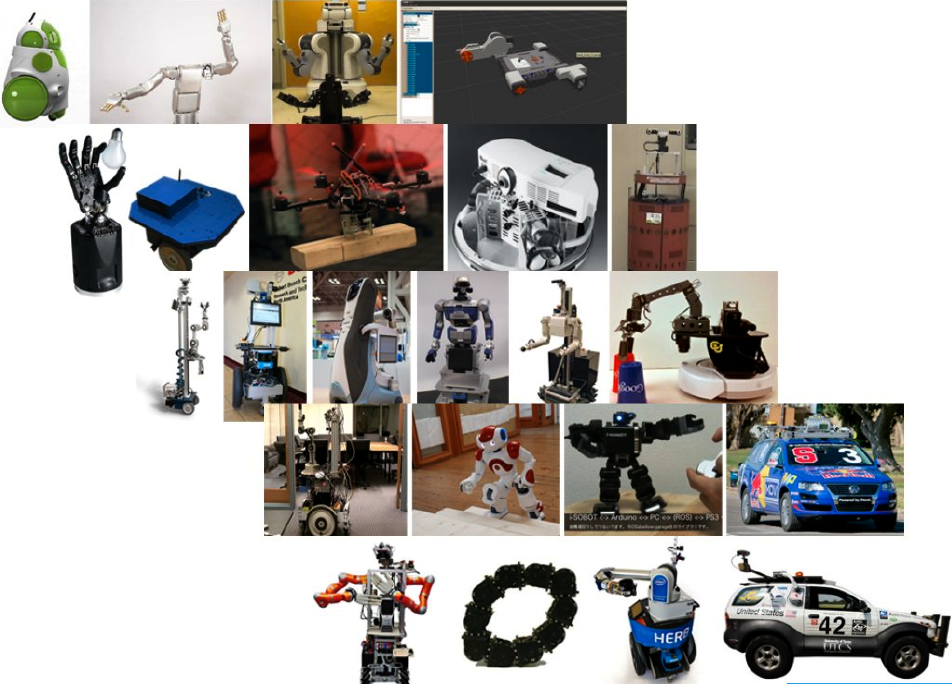
\includegraphics[bb=0bp -160bp 952bp 480bp,height=0.8\paperheight]{images/ROSManyRobots}
\end{figure}

\par\end{center}


\lyxframeend{}


\lyxframeend{}\lyxframe{ROS Basics}
\begin{itemize}
\item Supported Platforms

\begin{itemize}
\item Linux, Mac OS, partial support for Windows
\end{itemize}
\end{itemize}

\pause{}
\begin{itemize}
\item Languages

\begin{itemize}
\item C/C++, Python, Octave, Lisp, Java
\end{itemize}
\end{itemize}

\lyxframeend{}


\lyxframeend{}\lyxframe{What does ROS cover?}

\begin{minipage}[t]{0.45\textwidth}%
ROS
\begin{itemize}
\item Simulation
\item Task execution
\item Mobile manipulation
\item Navigation
\item Visualization
\item Client libraries
\item Message passing\end{itemize}
%
\end{minipage}%
\begin{minipage}[t][1\totalheight][c]{0.45\textwidth}%
\noindent \begin{center}

\includegraphics[width=1\columnwidth]{images/electric_200w_ROS}
\par\end{center}%
\end{minipage}


\lyxframeend{}


\lyxframeend{}\subsection{ROS Concepts}


\lyxframeend{}\lyxframe{ROS Nodes}
\begin{itemize}
\item Master (rosmaster)

\begin{itemize}
\item provides naming and registration services
\item tracks topics and services
\item enables localization of nodes (they talk peer-to-peer)
\item XML-RPC-based API
\end{itemize}
\item Generally: they are uniquely named
\end{itemize}

\lyxframeend{}


\lyxframeend{}\lyxframe{[allowframebreaks]ROS Communication}
\begin{itemize}
\item Publisher sends message to subscribers

\begin{itemize}
\item Usually TCP/IP transport
\item XML-RPC is only used to negotiate transport (no messages via XML-RPC)
\end{itemize}
\end{itemize}
\noindent \begin{center}
\begin{figure}[H]
\noindent \centering{}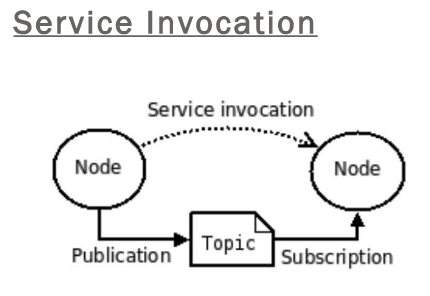
\includegraphics[width=0.45\textwidth]{images/ServiceInvocation}
\end{figure}

\par\end{center}


\lyxframeend{}


\lyxframeend{}\lyxframe{ROS Communication (cont.)}

\noindent \begin{center}
\begin{figure}[H]
\noindent \centering{}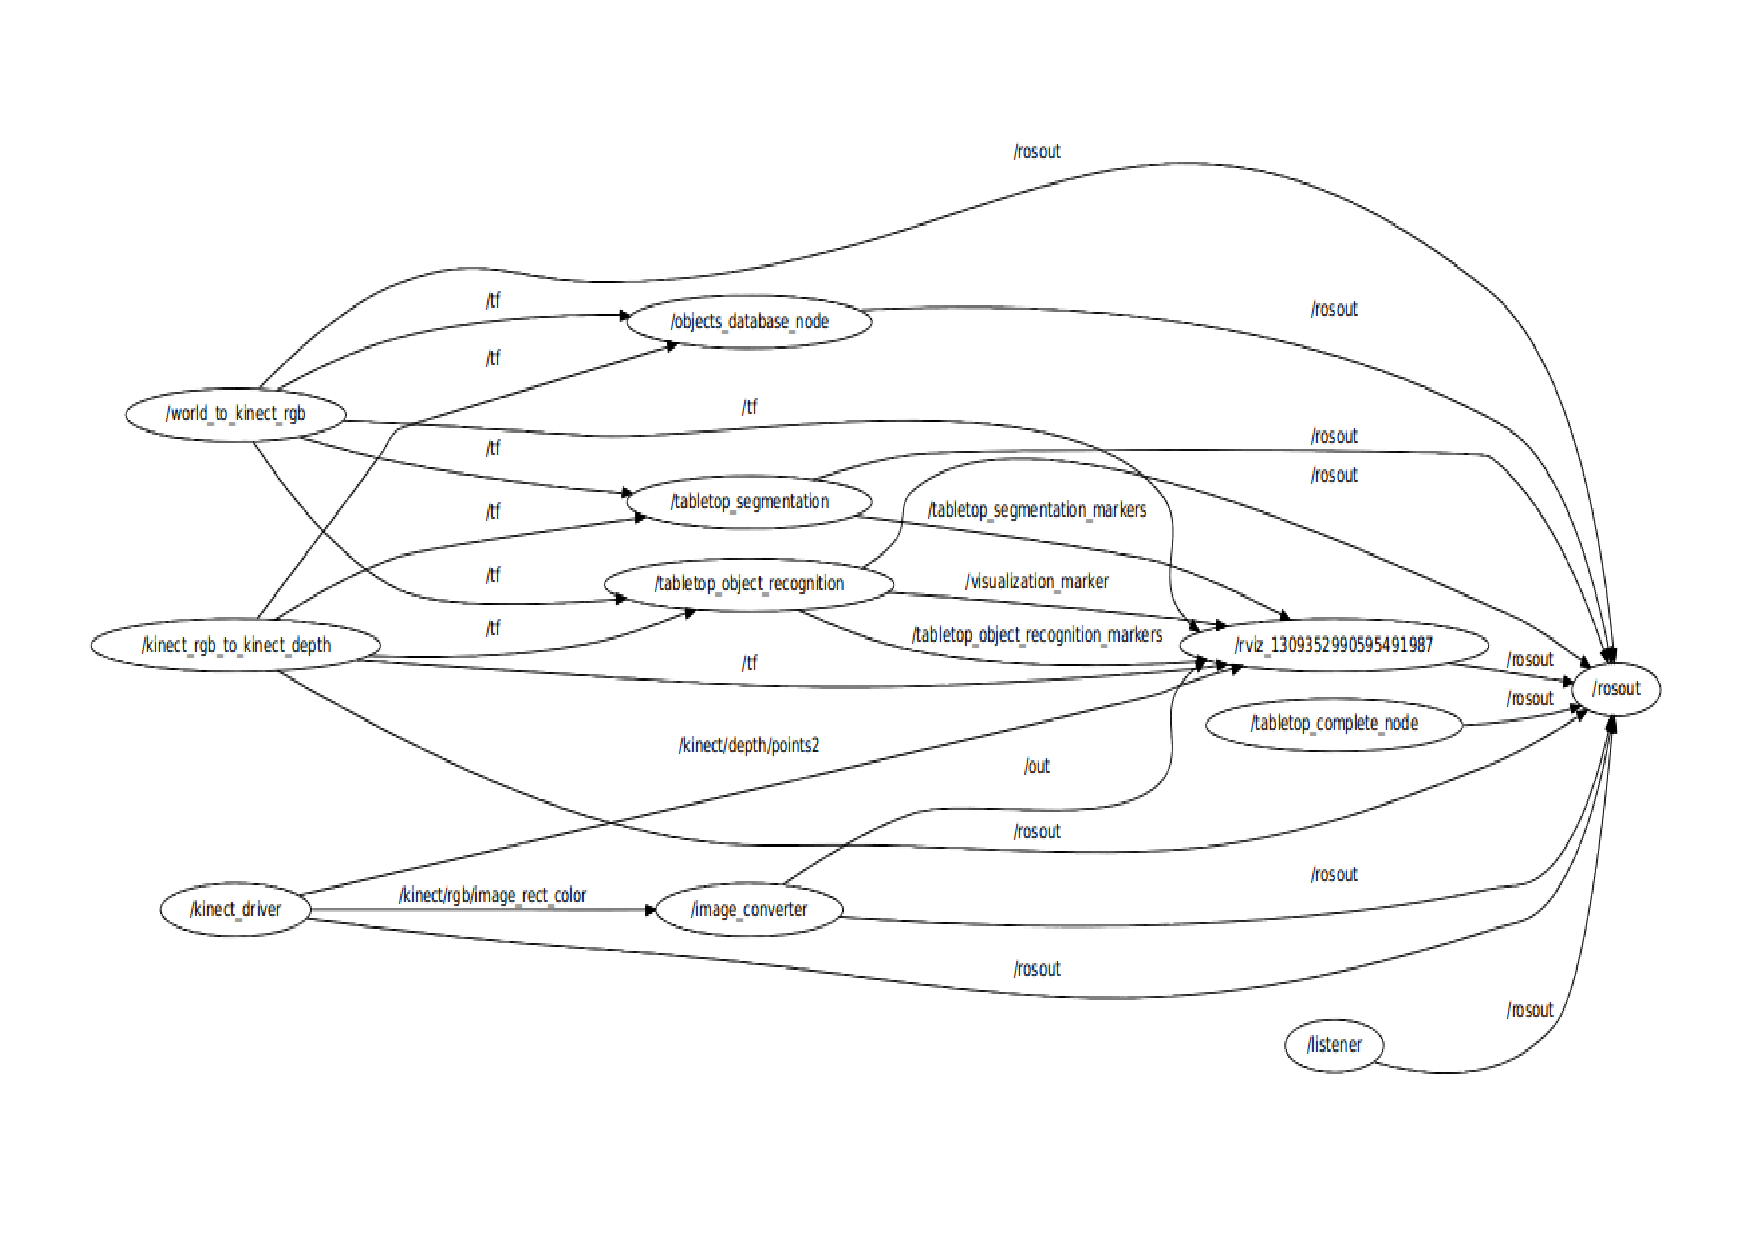
\includegraphics[bb=40bp 0bp 800bp 530bp,clip,width=1\textwidth]{images/ros_rxgraph}
\end{figure}

\par\end{center}


\lyxframeend{}


\lyxframeend{}\subsection{ROS Repositories}


\lyxframeend{}\lyxframe{ROS Repositories}

Repositories world-wide
\begin{itemize}
\item Collection of packages and stacks, hosted online
\item many repositories (>50): Stanford, CMU, TUM ..
\end{itemize}
\noindent \begin{center}
\begin{figure}[H]
\noindent \centering{}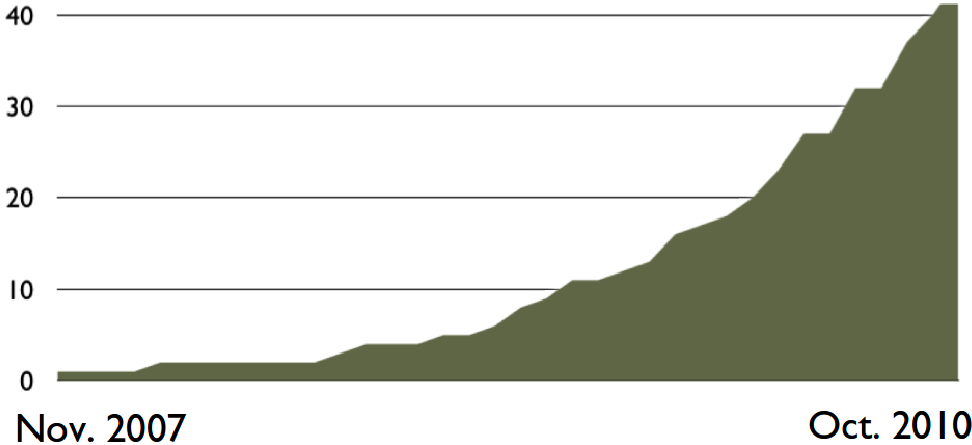
\includegraphics[width=0.9\textwidth]{images/ROSReopGrowth}
\end{figure}

\par\end{center}


\lyxframeend{}


\lyxframeend{}\lyxframe{ROS Repositories (cont.)}

\noindent \begin{center}
\begin{figure}[H]
\noindent \centering{}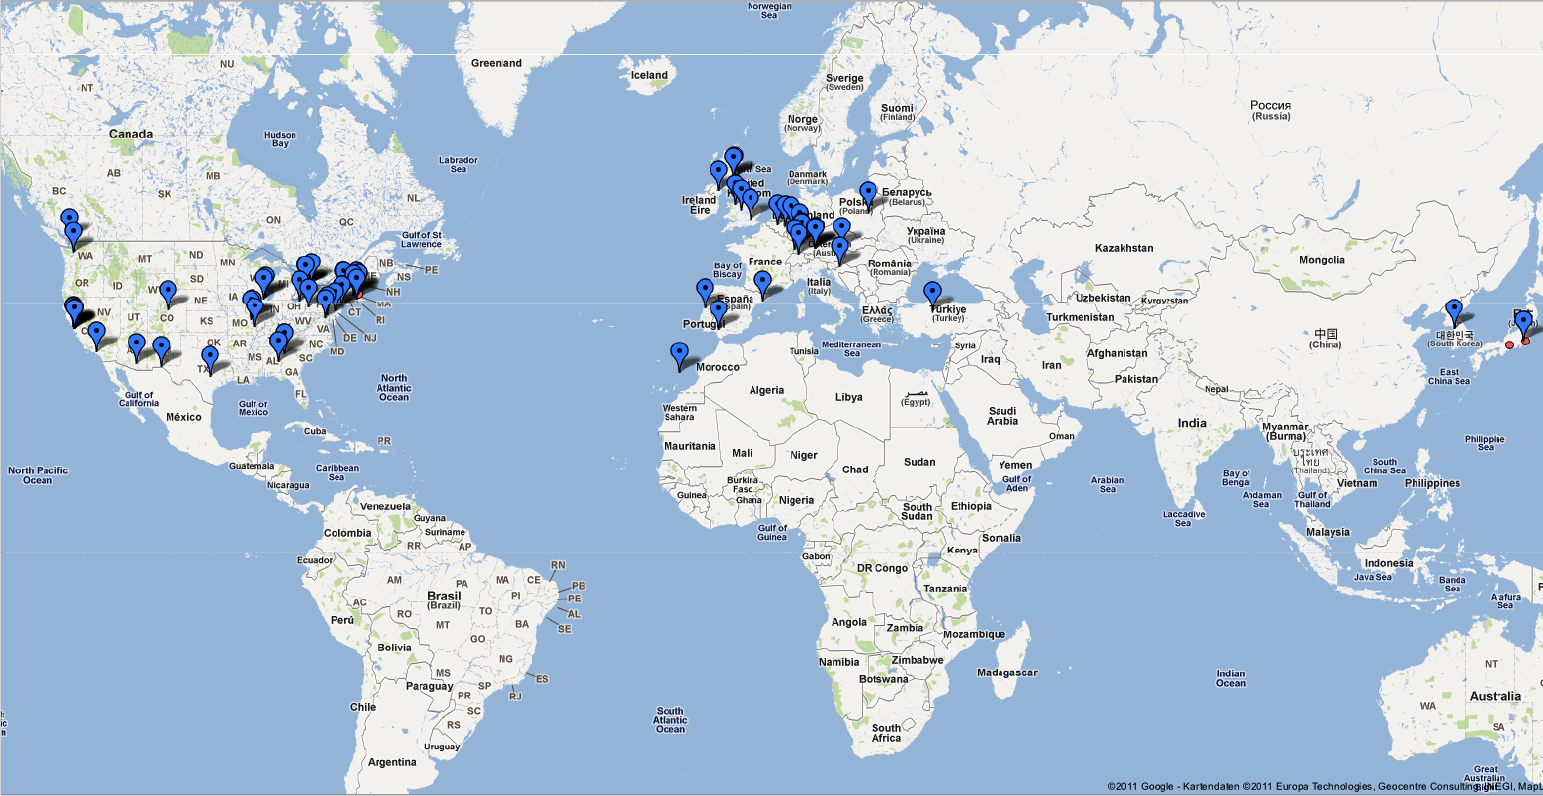
\includegraphics[bb=80bp 0bp 1350bp 550bp,width=1\paperwidth]{images/ROS_Repositories}
\end{figure}

\par\end{center}


\lyxframeend{}


\lyxframeend{}\lyxframe{ROS Stacks}
\begin{itemize}
\item Collect similar packages that work together to achieve e.g.:

\begin{itemize}
\item 2D Navigation
\item Manipulation
\item SLAM
\end{itemize}
\end{itemize}
\noindent \begin{center}
\begin{figure}[H]
\noindent \centering{}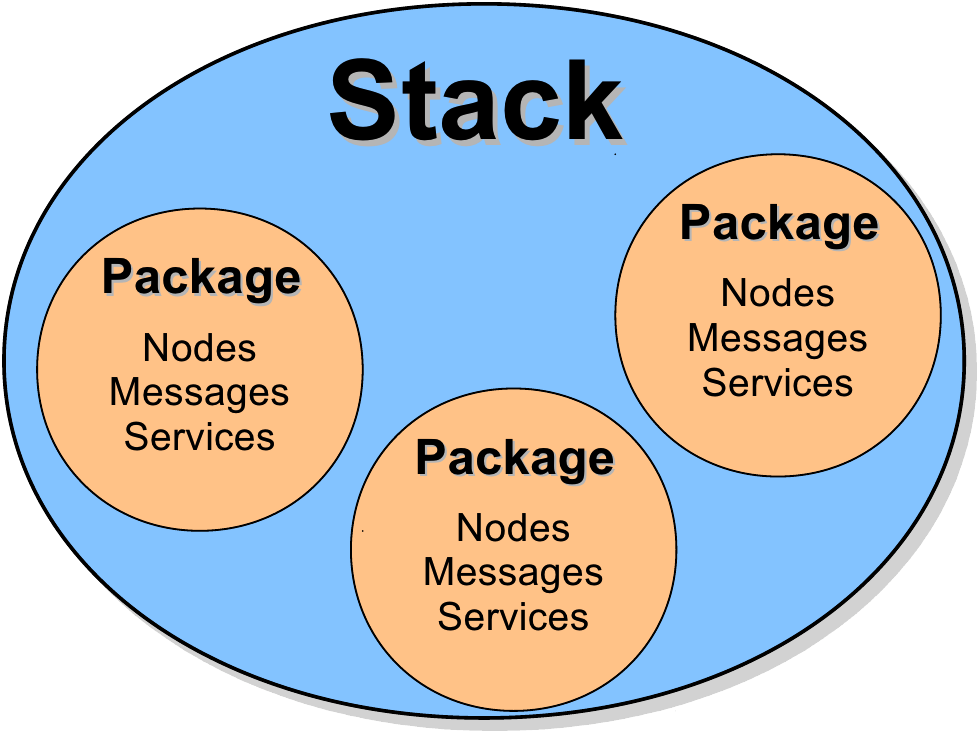
\includegraphics[width=0.45\textwidth]{images/ROSStack}
\end{figure}

\par\end{center}


\lyxframeend{}


\lyxframeend{}\lyxframe{ROS Stacks Overview%
\footnote{\href{http://www.ros.org/browse}{http://www.ros.org/browse}%
}}


\framesubtitle{Currently > 400 Stacks available}

\begin{minipage}[t]{0.45\textwidth}%
\begin{itemize}
\item (2D/3D) Navigation 
\item PR2 arm navigation
\item PR2 opening doors 
\item Exploration
\item GUI for PR2 robot
\item PR2 object manipulation 
\item PR2 simulator\end{itemize}
%
\end{minipage}%
\begin{minipage}[t]{0.5\paperwidth}%
\begin{figure}[H]
\noindent \centering{}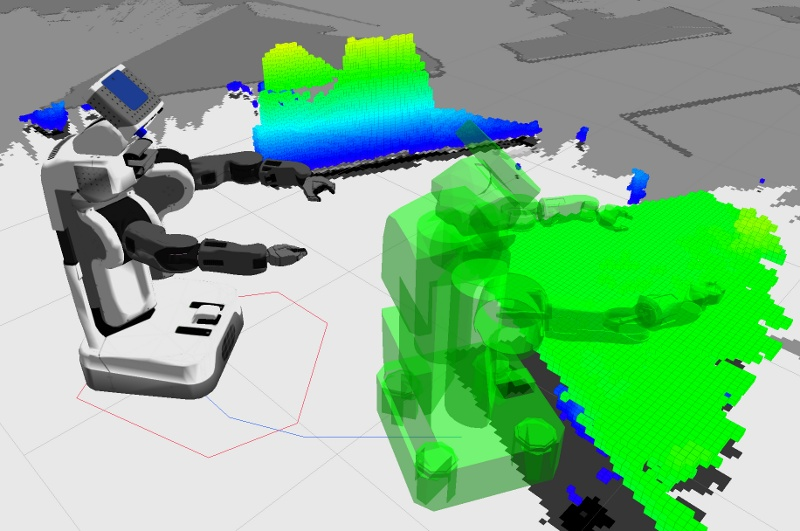
\includegraphics[height=0.4\textheight]{images/PR2_3DNavigation}\\
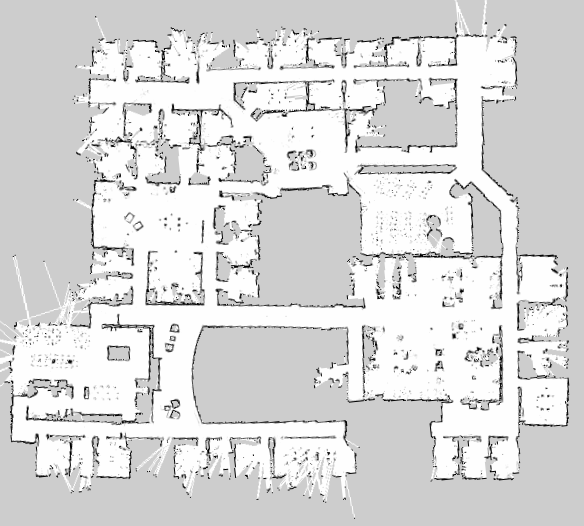
\includegraphics[height=0.2\textheight]{images/2DMapping}\includegraphics[height=0.2\textheight]{\string"images/PR2 Opening doors\string".png}
\end{figure}
%
\end{minipage}


\lyxframeend{}


\lyxframeend{}\lyxframe{ROS-based Navigation}

Includes
\begin{itemize}
\item Path planning, Obstacle avoidance, Automatic map making
\end{itemize}
\noindent \begin{center}
\begin{figure}[H]
\noindent \centering{}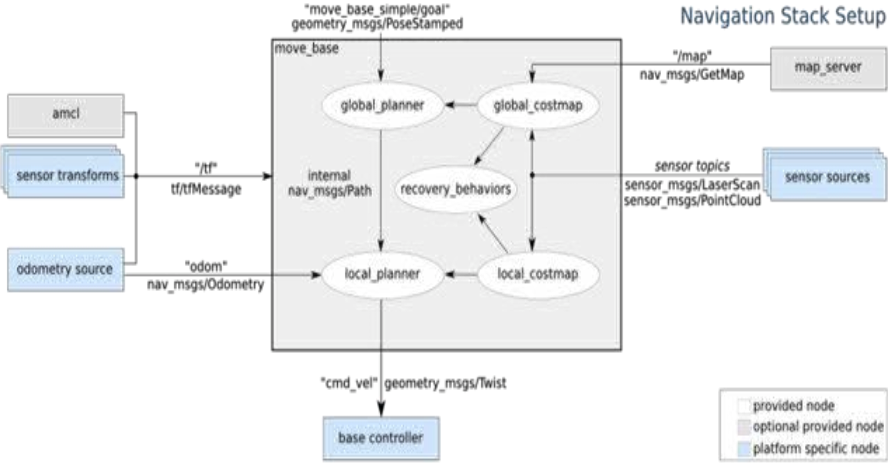
\includegraphics[width=0.9\textwidth]{images/ROSNavigation}
\end{figure}

\par\end{center}


\lyxframeend{}


\lyxframeend{}\lyxframe{[allowframebreaks]Example Application}

\noindent \begin{center}
\begin{figure}[H]
\noindent \centering{}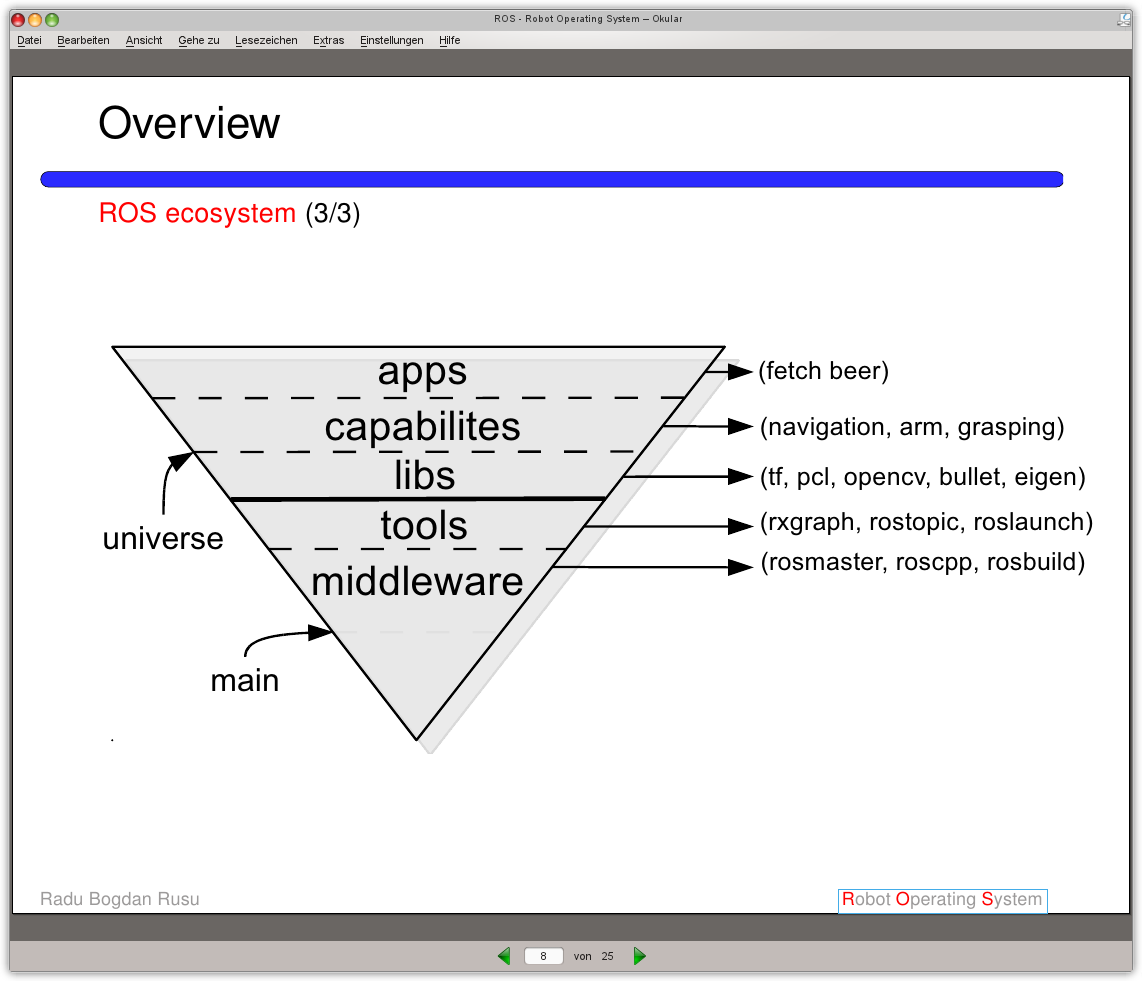
\includegraphics[width=1\textwidth]{images/ROSEcosystem}
\end{figure}

\par\end{center}
\begin{itemize}
\item universe - robot centric, main - general
\end{itemize}
\noindent \begin{center}
\begin{figure}[H]
\noindent \centering{}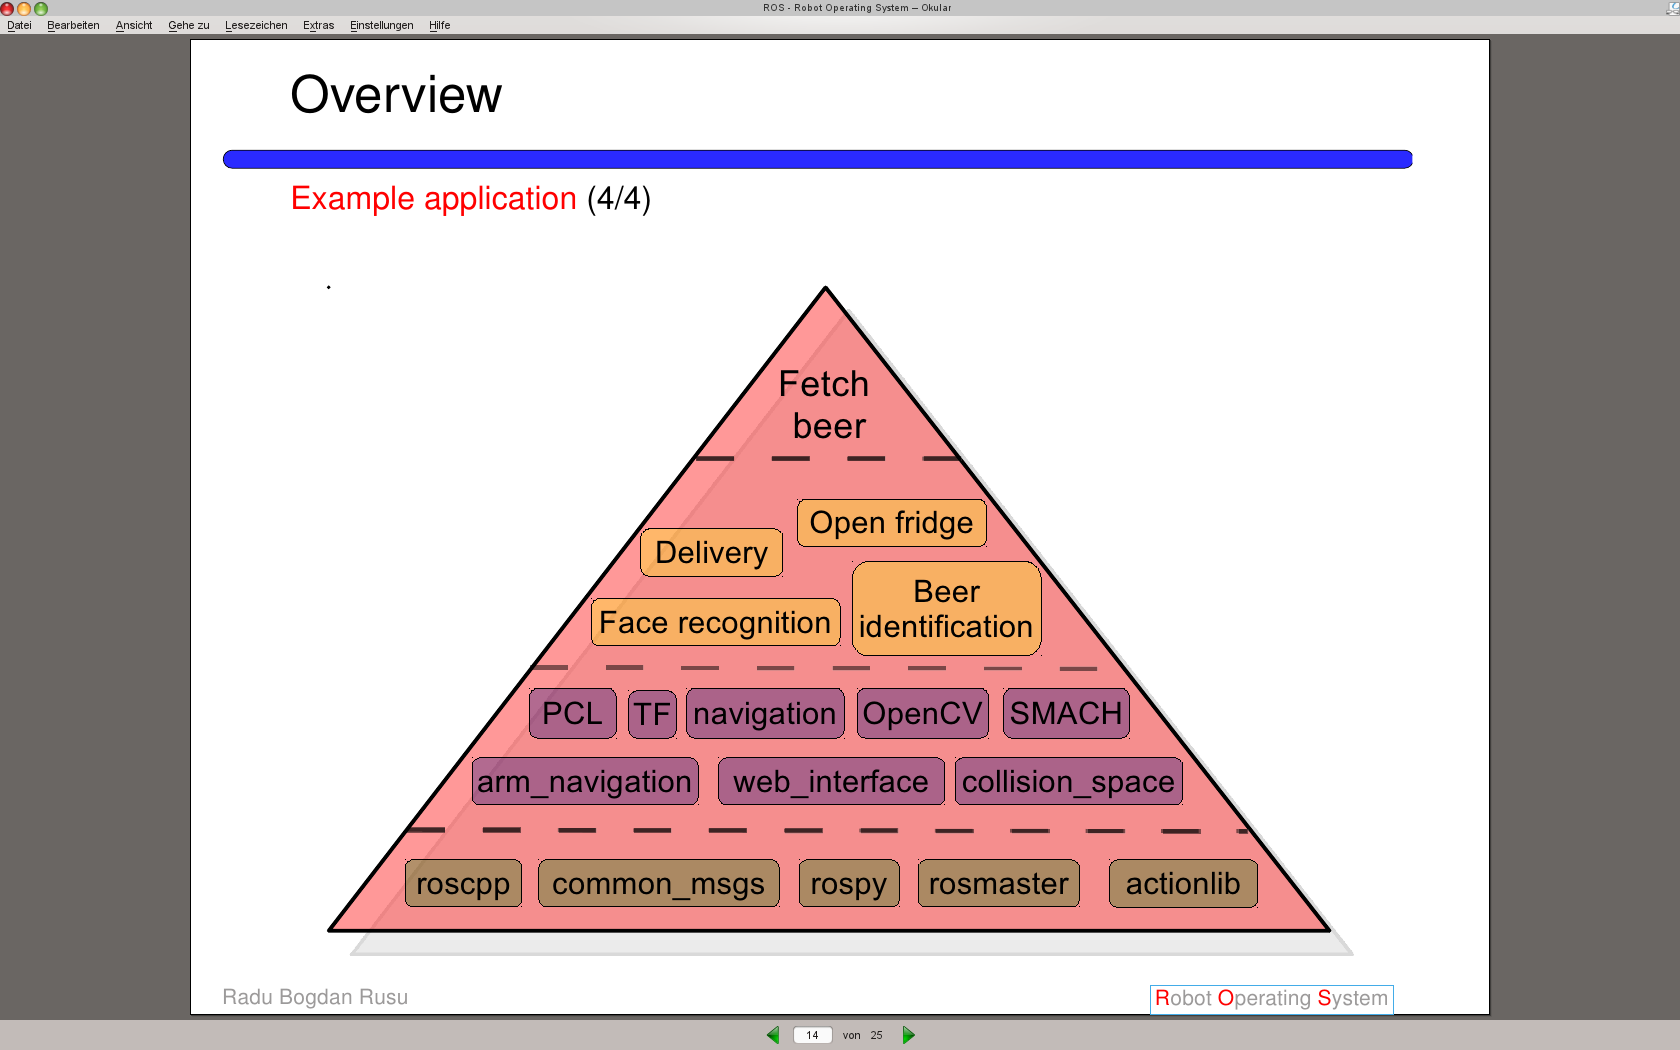
\includegraphics[width=0.9\textwidth]{images/ROSFetchBeer}
\end{figure}

\par\end{center}


\lyxframeend{}


\lyxframeend{}\lyxframe{ROS Strengths for RACE}
\begin{itemize}
\item Visualization
\item Object recognition
\item Navigation
\item Manipulation/Grasping
\item Plugging in Sensors

\begin{itemize}
\item already integrated
\item RACE specific
\end{itemize}
\end{itemize}

\lyxframeend{}




%%%%%%%%%%%%%%%%%%%%%%%%%%%%%%%%%%%%%%%%%%%%%%%%%%%%%%%
\section{Sensors and Simulation}
\subsection{Further Sensors}

\begin{frame} 
 \frametitle{Kinect}
\begin{itemize}
 \item Motion sensing input device by Microsoft for the Xbox 360 video game console
 \item Range camera technology by Israeli developer PrimeSense
 \item 3D scene information from a continuously-projected infrared structured light
\end{itemize}
\hspace{35ex}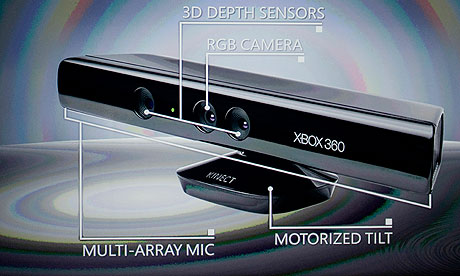
\includegraphics[width=5cm]{img/kinect.png}
\end{frame}

\begin{frame}
 \frametitle{Kinect operations - I}

\begin{itemize}
  \item The IR camera and the IR projector form a stereo pair with a baseline of approximately 7.5\,cm
  \item The IR projector sends out a fixed pattern of light and dark speckles
  \item The pattern is generated from a set of diffraction gratings, with special care to lessening the effect of zero-order propagation of a center bright dot
\end{itemize}
\hspace{35ex}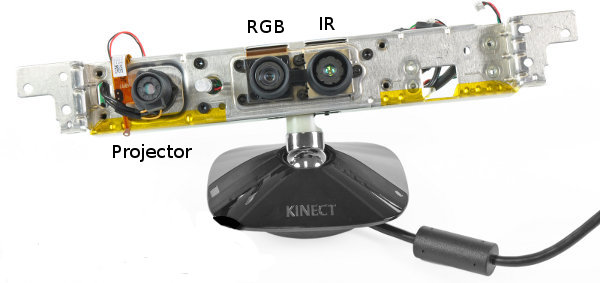
\includegraphics[width=5cm]{img/kinect2.png} 
\end{frame}

\begin{frame}
 \frametitle{Kinect - technical data}
\begin{itemize}
  \item Resolution of (640 $\times$ 480) @ 30 Hz (color) and (320 $\times$ 240) @ 30 Hz (depth)
  \item Angular field of view of $57^0$ horizontally and $43^0$ vertically
  \item Range of approximately 0.7 - 6\,m (practical 0.7 - 3.5\,m)
  \item Physical tilt range ($-31^0$  to $+31^0$ )
  \item Voice microphone and array supporting single speaker voice recognition (16-bit audio @ 16 kHz)
  \item OpenNI and Freenect drivers
\end{itemize}

\end{frame}


\begin{frame} 
 \frametitle{Kinect - first results}
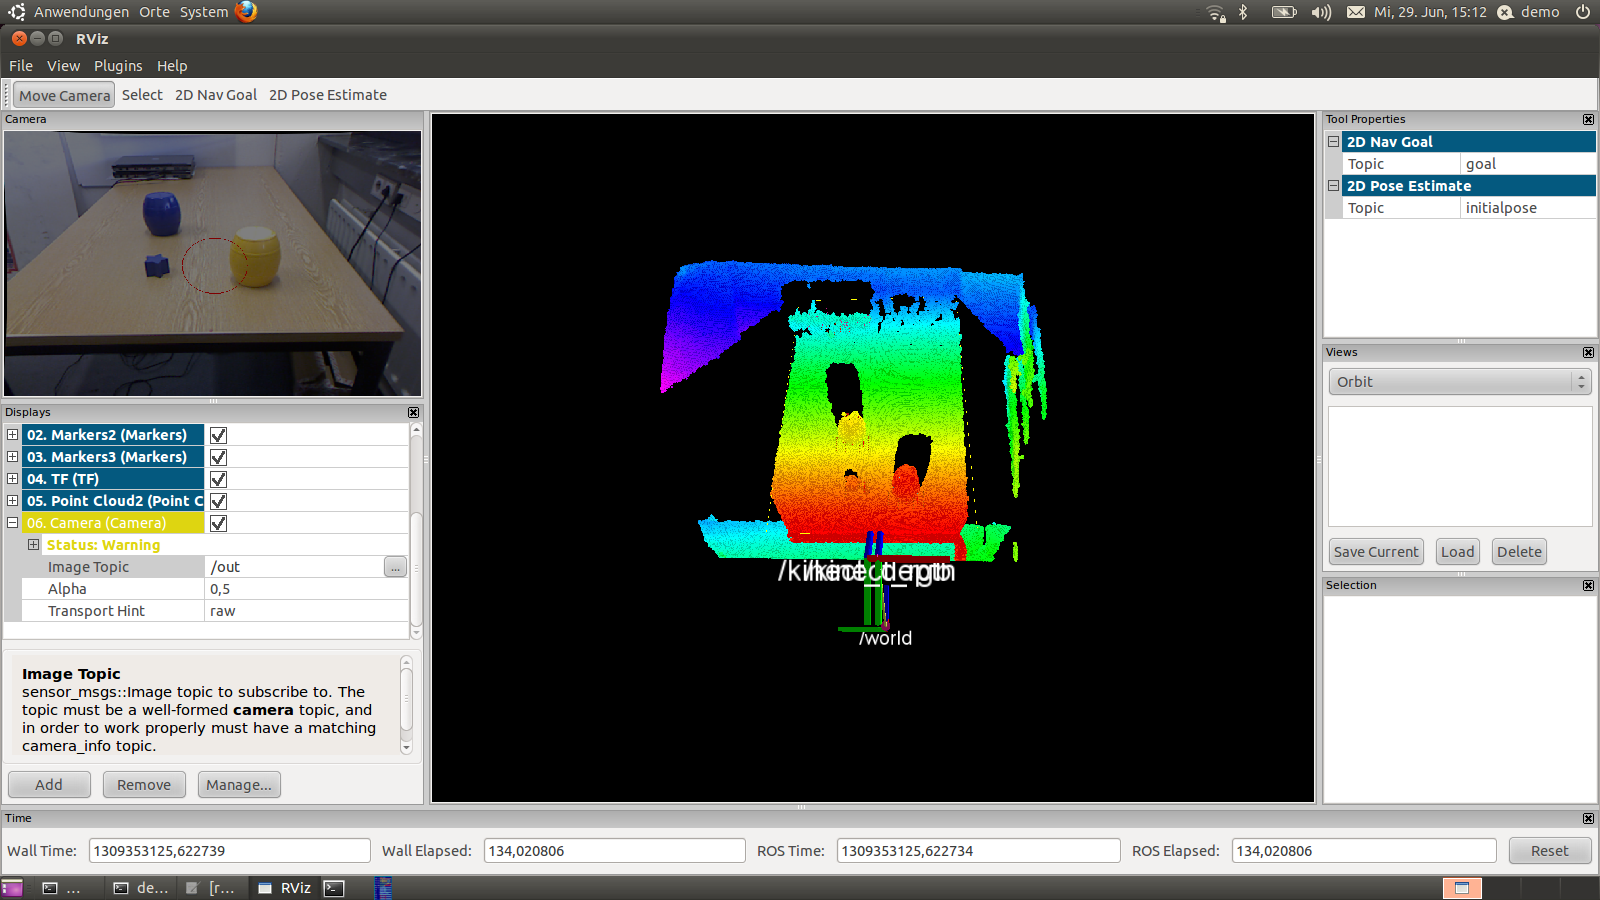
\includegraphics[width=11cm]{img/ros_rviz.png}
\end{frame}


\begin{frame}
 \frametitle{Kinect - summary}
\begin{itemize}
  \item Fast sensor with large resolution
  \item Stable, repeatable results
  \item Ideal for surfaces, inaccuracy on edges (remedy through fusion with the tof-camera (200 $\times$ 200 @ 40 fps) or other sensors)
\end{itemize}
\hspace{3ex}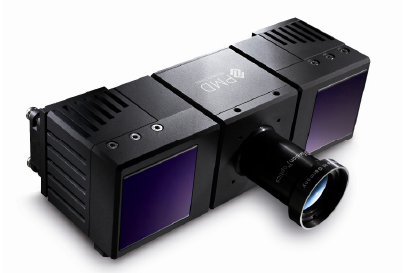
\includegraphics[width=5.5cm]{img/camcube.png}
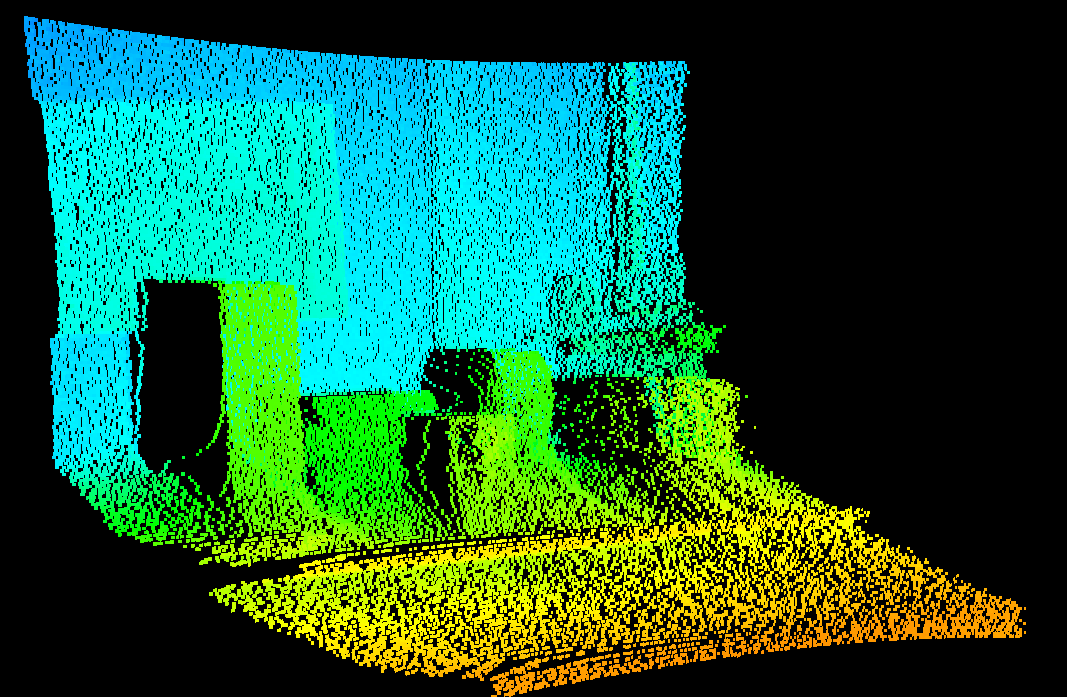
\includegraphics[width=5.5cm]{img/pmd2.png}
\end{frame}

\begin{frame}
 \frametitle{PMD Camcube in ROS}
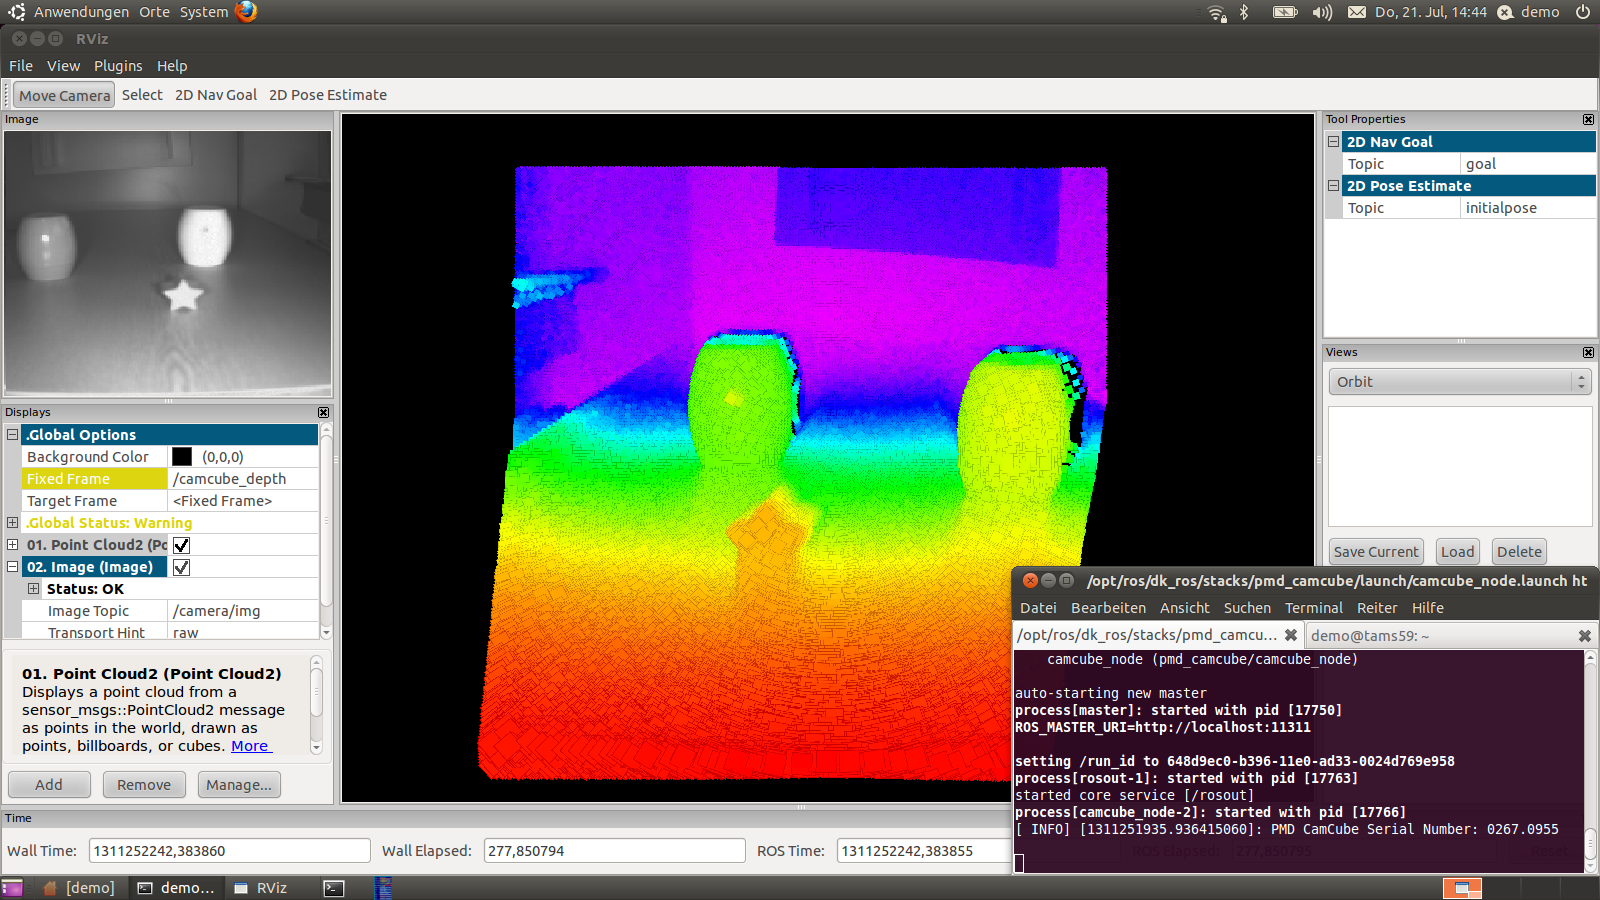
\includegraphics[width=11cm]{img/camcube_ros.png}
\end{frame}

\begin{frame}
 \frametitle{FLIR A615}
\begin{itemize}
  \item FOV $25^0 \times 19^0$
  \item IR resolution $[640 \times 480]@50$ Hz
  \item Accuracy $\pm 2^0\,C$ or $\pm 2\%$ of reading
  \item Image and control over Gigabit Ethernet
\end{itemize}

\vspace{5ex}\hspace{37ex}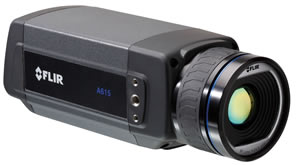
\includegraphics[width=4cm]{img/A615_300.jpg}
\end{frame}

\begin{frame}
 \frametitle{FLIR A615}
\vspace{-1ex}{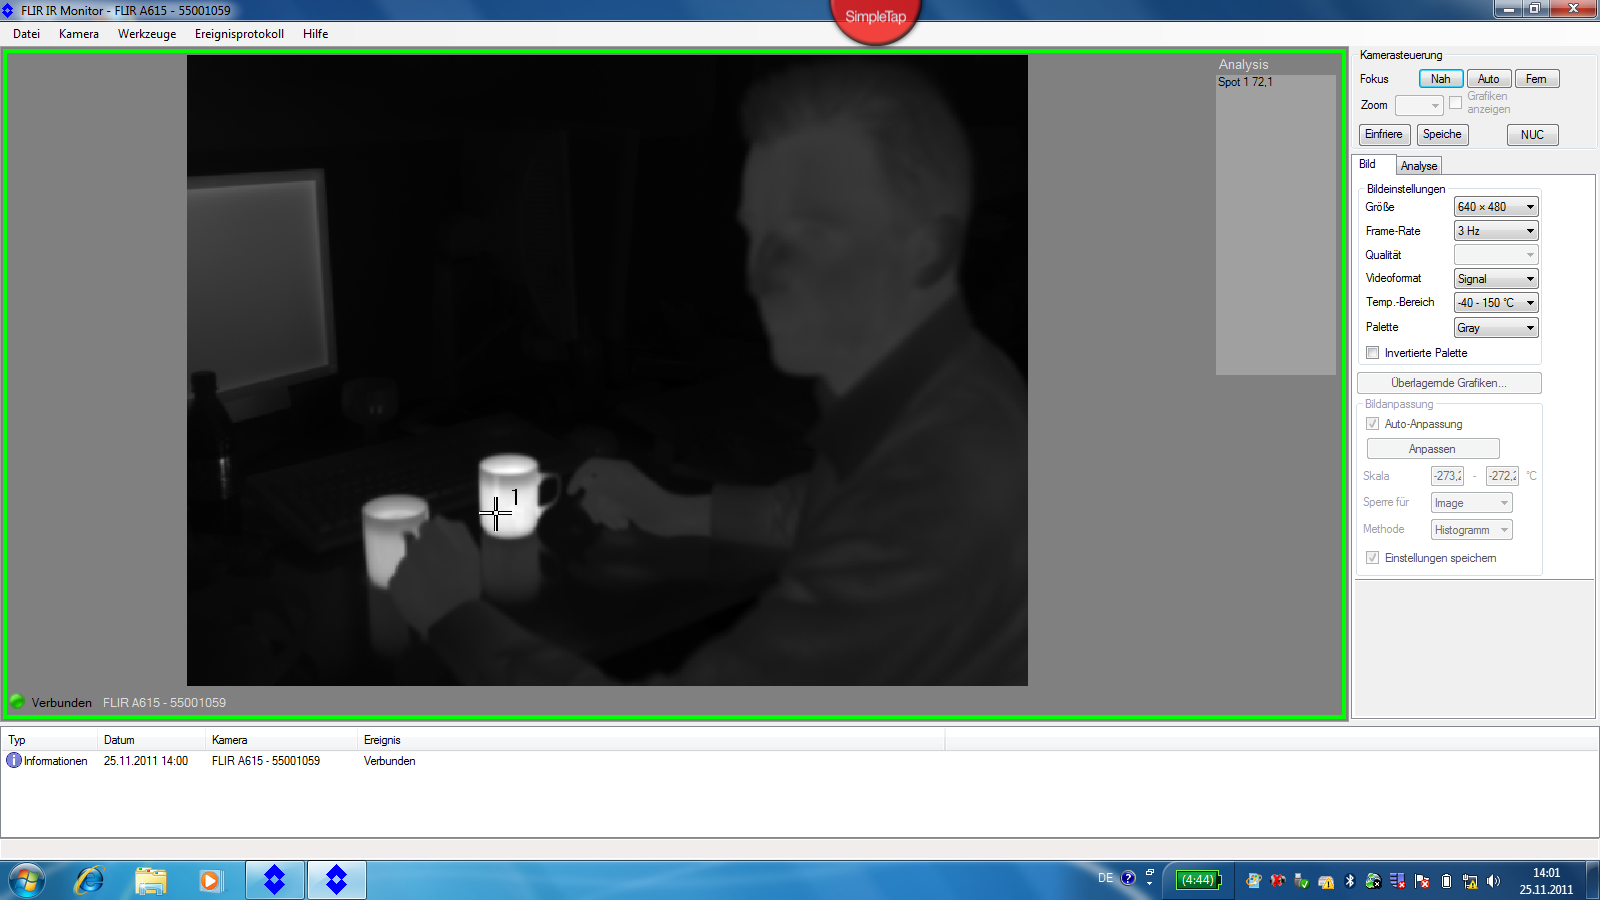
\includegraphics[width=7cm]{img/hannes_flir.png} \\
\vspace{-7ex} \hspace{22ex}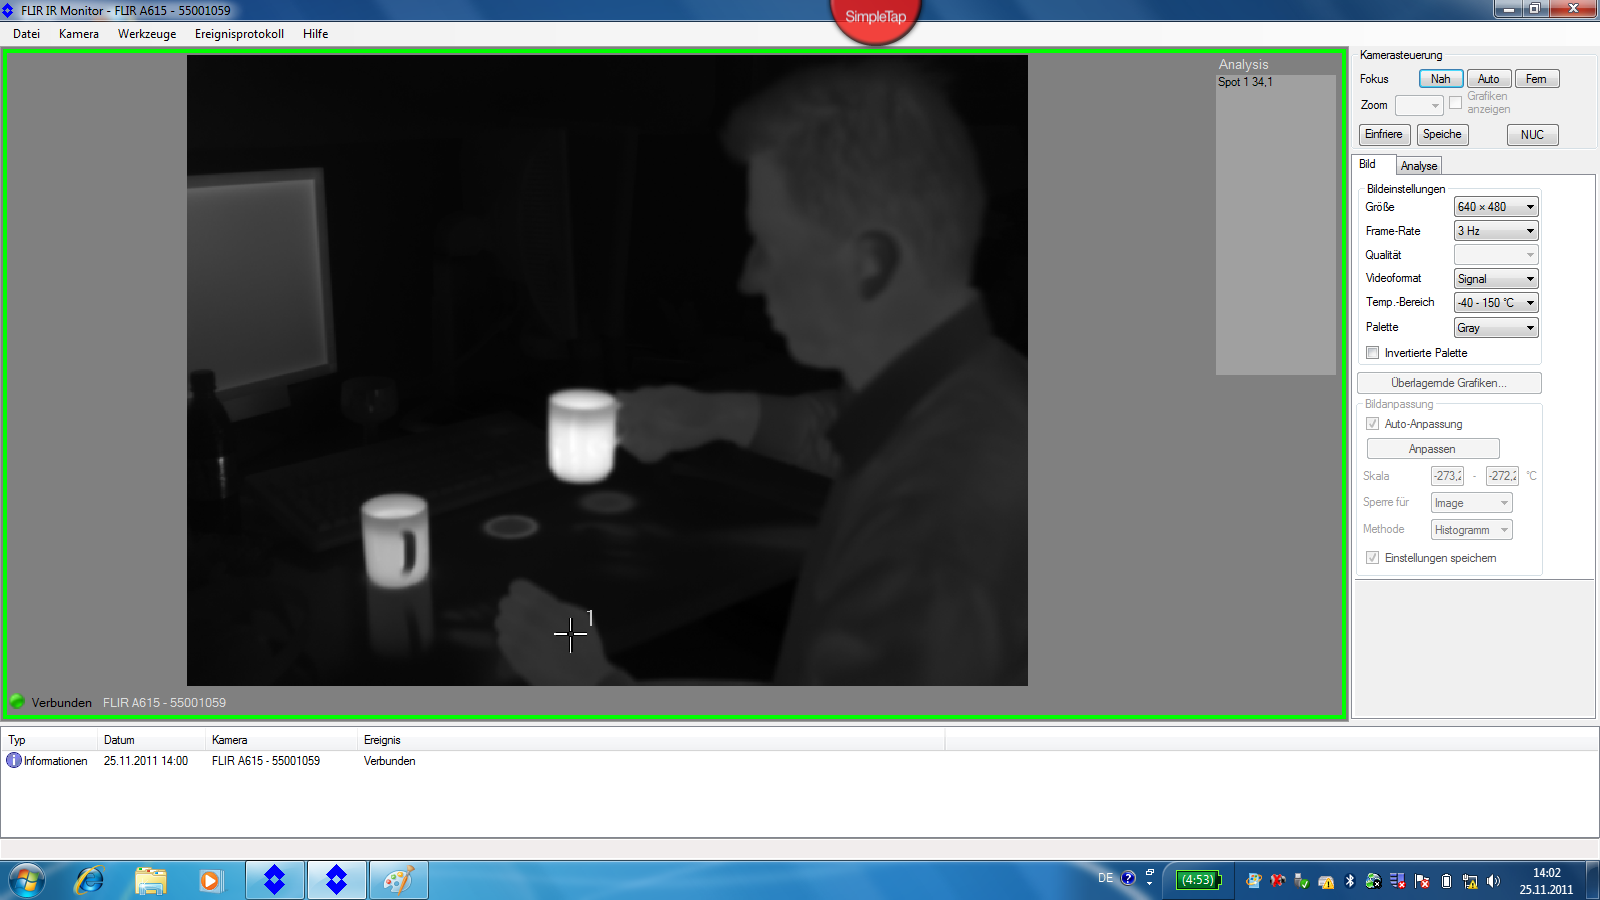
\includegraphics[width=7cm]{img/hannes_flir2.png}
}
\end{frame}

\subsection{Gazebo} % - 3D dynamic multi-robot simulation
% intro / abstract etc.			--------------------------------------
\begin{frame}
  \frametitle{Gazebo}
\begin{itemize}
    \item Developed to be fully compatible with the Player\footnote{The Player/Stage Projekt, http://playerstage.sourceforge.net/} device server
    \item Full integrated in ROS (version 1.0)
    \item 3D dynamic multi-robot simulation
    \item Open source
    \item ODE -  Open Dynamics Engine (Bullet)

   
\end{itemize}
\end{frame}

\begin{frame}
  \frametitle{Gazebo}
\begin{itemize}
    \item The World represents the set of all models and environmental factors such as gravity and lighting
    \item Accuracy in terms of robot sensors and actuators
    \item API for easily create new robots, actuators, sensors, and arbitrary objects
    \item Possibilities to create complex worlds
    \item Simulation of remote environments
    \item GUI for data visualization
    \item Visualization with help of OpenGL and GLUT
    
\end{itemize}
\end{frame}

\begin{frame}
  \frametitle{General Structure of Gazebo components}
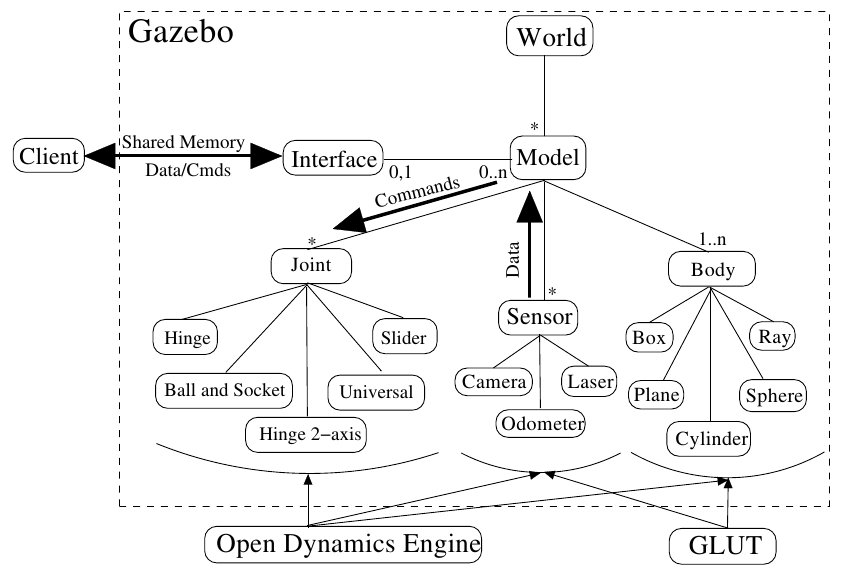
\includegraphics[width=9cm]{img/gazebo_struktur.png}
\end{frame}

\begin{frame}
  %\frametitle{}
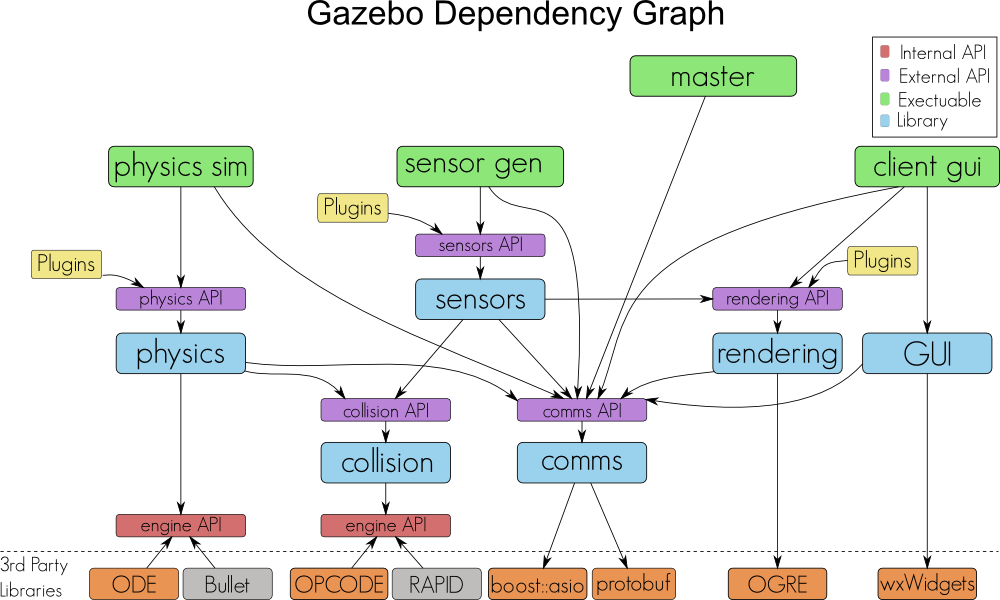
\includegraphics[width=11cm]{img/gazebo_dependency_graph.png}
\end{frame}

\begin{frame}
  \frametitle{ROS Simulation Interface}
\hspace{5ex}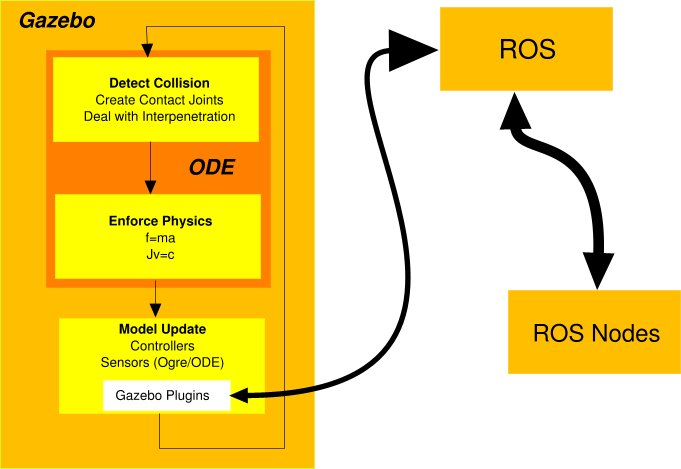
\includegraphics[width=9cm]{img/ros_simulation_interface.jpg}
\end{frame}

\begin{frame}
  \frametitle{ROS, Stage, PR2}
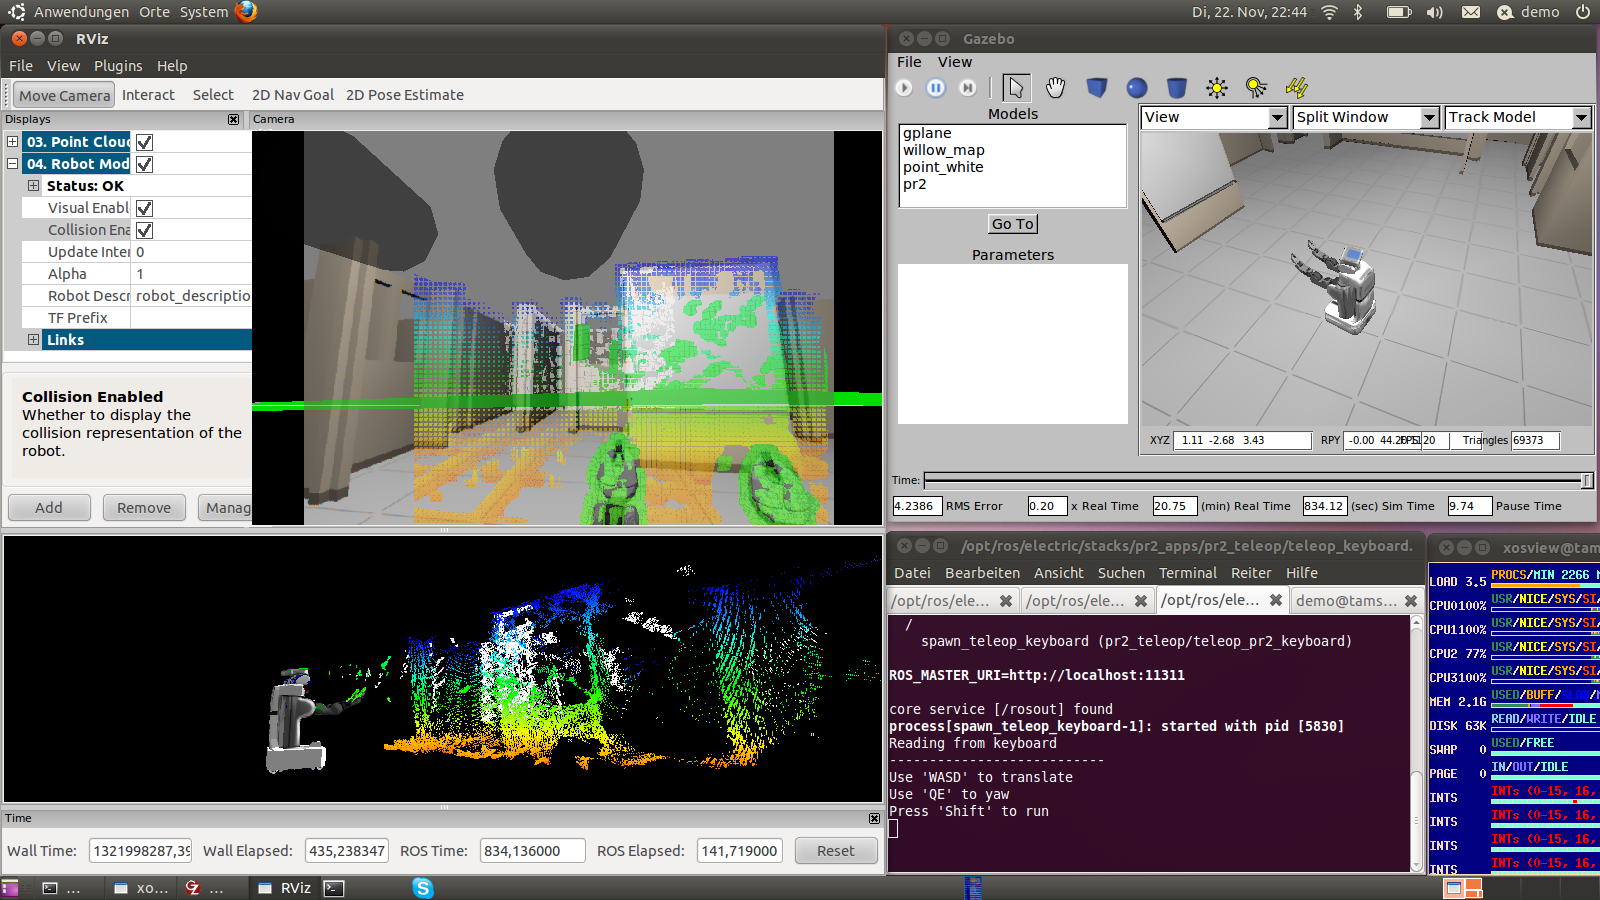
\includegraphics[width=11cm]{img/race_pr2_ros_rviz2.png}
\end{frame}
%%%%%%%%%%%%%%%%%%%%%%%%%%%%%%%%%%%%%%%%%%%%%%%%%%%%%%%




\appendix

\lyxframeend{}\section*{}


\lyxframeend{}\section*{Appendix}


\lyxframeend{}\lyxframe{Thank You!}

\begin{center}
{\LARGE Any questions?}
\par\end{center}{\LARGE \par}


\lyxframeend{}


\lyxframeend{}\subsection*{Further Reading}


\lyxframeend{}\lyxframe{[allowframebreaks]Further Reading}





\bibliographystyle{alpha}
\bibliography{/Users/sebastian/Documents/_BibPapers/Rockel,/Users/sebastian/Documents/_BibPapers/Agent2010,/Users/sebastian/Documents/_BibPapers/ICRA2009,/Users/sebastian/Documents/_BibPapers/ICRA2010,/Users/sebastian/Documents/_BibPapers/IROS2009,/Users/sebastian/Documents/_BibPapers/IROS2010,/Users/sebastian/Documents/_BibPapers/ISR2010,/Users/sebastian/Documents/_BibPapers/ModRobots2009,/Users/sebastian/Documents/_BibPapers/Robotics2009,/Users/sebastian/Documents/_BibPapers/Robotics2010,/Users/sebastian/Documents/_BibPapers/RoboticsGeneral,/Users/sebastian/Documents/_BibPapers/ICRA2009}



\lyxframeend{}

\end{document}
